\label{Appendix:pixels_overview}
\section{Signal formation}
    When a charge particle passes through a pixel and loses energy by ionization a part of that energy is used to generate electron-hole pairs (an other part is used for other processes, as the lattice excitation) which are then separated by the elettric field and collected at their respectivelly electrodes ($p$ for holes and $n$ for electrons)\footnote{Even if in principle both the electrode can be used to read a signal, for pixel detectors, where the number of channel and the complexity of readout are high, only one is actually used. In strip and pad detectors, instead, is more common a dual-side readout}; by the drift of these charges, a signal $i_e$ is generated on the  electrode $e$ as stated by the Shockley–Ramo's theorem: 
    \begin{equation}
        i_e(t) = -q\: v(t)\, E_{WF,e}
    \end{equation}
    where $v(t)$ is the instantaneous velocity of the charge $q$ and $E_{WF}$ is the weighting field, that is the field obtained biasing the electrode $e$ with 1V and all the others with 0V.\\
    The drift velocity of the charge depends on the elettric field and on the mobility of the particle:
    \begin{equation}
        v = \mu(E)\, E
    \end{equation}
    where $\mu(E)$ is a function of the electric field and is linear with $E$ only for small $E$: at highter values the probability of interactions with optical phonons increases and the mobility drops and this leads to an indipendency of the velocity from the electric field (fig. \ref{fig:mobility_drift2}).\\
    SECONDO ME MANCA ANCORA UNA FRASE DI CONNESSIONE\\
    \begin{figure}[h!]
        \begin{subfigure}{.5\textwidth}
        \centering
        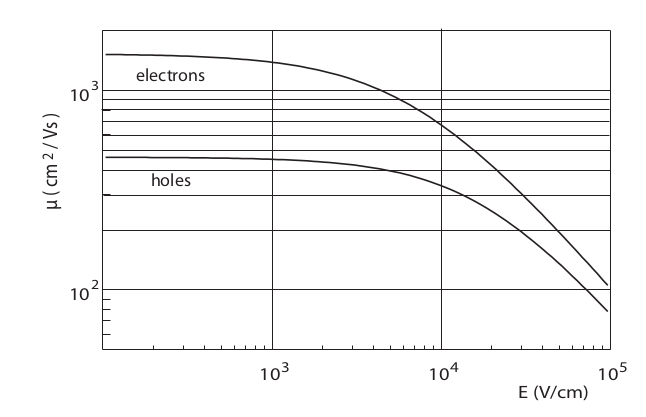
\includegraphics[width=.8\linewidth]{figures/overview/mobility_in_semiconductor.png}
        \caption{Typical values for elecrons and holes mobility 
        in silicon at room temperature are $\mu _n \sim$ 1450 $cm^2/Vs$, $\mu _h = 500$}
        \label{fig:mobility_drift1}
        \end{subfigure}
        \begin{subfigure}{.5\textwidth}
        \centering
        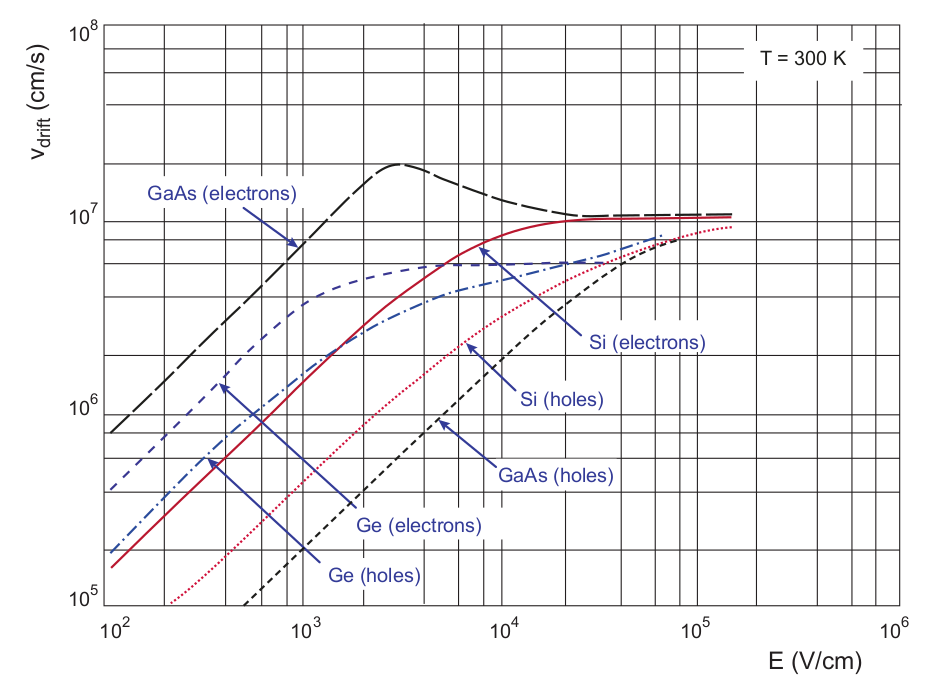
\includegraphics[width=.8\linewidth]{figures/overview/velocity_in_semiconductor.png}
        \caption{Drift velocity at room temperature in different semiconductors}
        \label{fig:mobility_drift2}
        \end{subfigure}
        \label{fig:mobility_drift}
    \end{figure}

    The average energy needed to create a pair at 300 K in silicon is $w_i$ = 3.65 eV, that is more than the mean ionization energy because of the interactions with phonon, since for a minimum ionizing particle (MIP) the most probable value (MPV) of charge released in the semiconductor is 0.28 keV/$\mu$, hence the number of e/h pairs is: 
    \begin{equation}
        \langle \frac{dE}{dx}\rangle \frac{1}{w_i} \sim 80 \: e/h \sim \frac{1.28 \:10^{-2}fC}{\mu m}
    \end{equation}
    CON UN'INCERTEZZA CHE È RADICE DI N; ED EVENTUALEMTNE SI AGGIUNGE IL FATTORE DI FANO NEL CASO DI ASSORBIMENTO TOTALE. iL FATTORE DI FANO È 0.115 NEL SILICIO\\ 
    It is foundamental that pairs e/h are produced in the depleted region of the semiconductor where the probability of recombination with charge carriers is low to avoid loss of signals.\\
    Pixel detectors are then commonly reverse biased: a positive bias is given to the $n$ electrode and a negative to the $p$
    to grow the depletion zone in the epitaxial layer below the electrode. The width of the depletion region is related with the extern bias $V_{ext}$, the resistivity $\rho$ and also with the dopant:
    \begin{multicols}{2}
        \begin{equation}
            d_{n} \sim 0.55 \sqrt{\frac{\rho}{\Omega cm}\frac{V_{ext}}{V}} \mu m 
        \end{equation}\break
        \begin{equation}
            d_{p} \sim 0.32 \sqrt{\frac{\rho}{\Omega cm}\frac{V_{ext}}{V}} \mu m
        \end{equation}
        \label{eq:deplation_d}
    \end{multicols}
    DA DOVE VENIVA QUESTA DIFFERENZA? DALLA MOBILITÀ MA NON MI RICORDO COME CI SI ARRIVAVA.\\
    For that reason high resistivities wafer (100 $\Omega cm - k\Omega cm$) are typically prefered beacause they allow bigger deplation zone with smaller voltage bias. 

\section{Radiation dameges}
    Radiation hardeness is a fundamental requirement for pixels detector especially in HEP since they are almost always installed near the interaction point where there is a high energy level of radiation. At LHC the $\phi_{eq}$ per year in the innermost pixels detector is $10^{14} n_{eq}/cm^2$; this number reduces by an order passing to the outer tracker layer. (referenza: pag 341 Wermes)\\ 
    Here the high fluence of particles can cause a damage both in the substrate of the detector and in the superficial electronics. 
    
    The first one has a principal non ionising nature (non ionizing energy loss, NIEL) since it is related with the dislocation of the lattice caused by the collision with nuclei; by this fact the NIEL hypothesis states that the substrate damage is normalized to the damage caused by 1 MeV neutrons. Differently, surface damages are principally due to ionising energy loss.

    DUE PAROLE IN PIÙ SUL SURFACE DAMAGE\\
    a charge accumulation in oxide ($S_iO_2$) can cause the generation of parasitic current with an obvious increase of the 1/f noise.\\
    Anyway surface damages are less relevant then the previous one since with the development of microelectronics and with the miniaturization of components (in electronic industry 6-7 nm transistors are already used, while for MAPS the dimensions of components is around 180 nm) the quantity of oxide in circuit is reduced.

    Let's spend instead two more other words on the more-relevant substrate damages: the general result of high radiation level is the creation of new energy levels within the silicon band gap and depending on their energy-location their effect can be different, as described in the Shockely-Read-Hall (SRH) statistical model.
    \begin{figure}
        \begin{subfigure}{.5\textwidth}
        \centering
        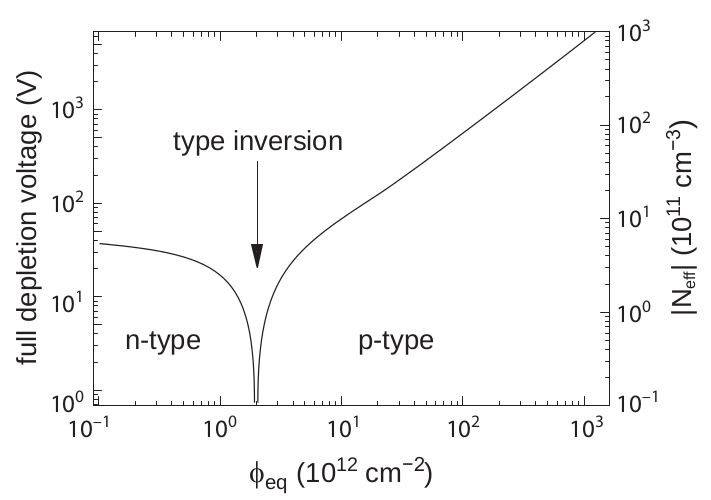
\includegraphics[width=.8\linewidth]{figures/overview/type_inversion.png}
        \caption{1a}
        \label{fig:type_inversion}
        \end{subfigure}%
        \begin{subfigure}{.5\textwidth}
        \centering
        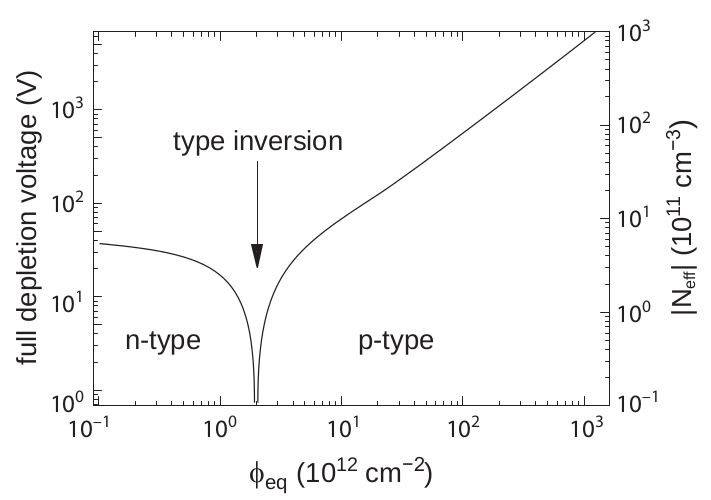
\includegraphics[width=.8\linewidth]{figures/overview/type_inversion.png}
        \caption{1b}
        \label{fig:type_inversion}
        \end{subfigure}
    \end{figure}
    The three main consequence of radiation damages are the changing of the effect doping concentration, the leakage current and the increasing of trapping probability.

    \textbf{Changing of the effective doping concentration:} is associated with the creation/removal of donors and acceptors center which trap respectively electrons/holes from the conduction band and cause a change in effective space charge density. Even an inversion (p-type becomes n-type\footnote{L'INVERSIONE OPPOSTA NON CE L'HAI PERCHÈ L'INVERSIONE È ASSOCIATA AD UN CAMBIO DELLA CONCETRAZIONE DA ... A ...\\E COME MAI L'ALTRO NON È FAVORITO?}) can happen: indeed it is quite common and happens at not too high fluences ($\phi_{eq} 10^{12-13}n_{eq}cm^{-2}$). 
    A changing in the doping concentration requires an adjust of the biasing of the sensor in time (eq.\ref{eq:deplation_d}) and sometimes can be difficult keeping to fully deplete the bulk.

    \textbf{Leakage current:} is associated with the generation-recombination centres. It has a strong dependence with the temperature ($I_{leak}\propto T^2$), whose solution is therefore to operate at lower temperature.

    \textbf{Increase of trapping probability:}  È ASSOCIATA CON QUALE TIPO DI CREAZIONE DI LIVELLO ENERGETICO?
    since the trapping probability is costant in the depleted region, the collected charge decreases exponentially with the drift path. The exponential coefficient, that is the mean trapping path, decreases after irradiation and typical values are 125-250 $\mu m$ and must be compared with the thickness of the depleted region which () corresponds to the mean drift path.

    Different choises for substate resistivity, for junctions type and for detector design are typically made to fight radiation issues. Some material with high oxygen concentration (as crystall produced using Czochralki (Cz) or float-zone (Fz) process (CONTROLLA SE SONO LORO QUELLI GIUSTI)) for example, show a compensation effect for radiation damage; an other example is the usage of n+ -in-p/n sensors (even if p+ -in-n sensors are easier and chieper to obtain) to get advantage of inversion/to have not the inversion (since they are already p-type). After inversion the n+p boudary, coming from n+ in-n, but to keep using the sensor the depletion zone still must be placed near the diode\footnote{With inversion some isolation process of electrodes can become important and p-spray/p-stop tecnique can eventually be applied. PERCHÈ CON L'INVERSIONE TI POTREBBE SERVIRE UNA TECNICA DI ISOLAMENTO?}.
    
    
    Radiation damage in CMOS circuits is entirely due to charge
    carriers generated by ionization in the dielectric layers of the
    process